\documentclass[12pt]{article}
\usepackage{float}
\usepackage{sbc-template}
\usepackage{graphicx,url}
\usepackage[brazil]{babel}   
\usepackage[utf8]{inputenc} 
\usepackage{verbatim}
\usepackage{tabularx}
\usepackage{array}

% pacote para citações entre aspas
\usepackage{dirtytalk}
     
% Tabela com linhas de espessuras diferentes
\usepackage{booktabs}

% Colunas de largura fixa, com diversos alinhamentos do texto (centralizado, direita, esquerda)
% Exemplo de uso: C{2.5cm}
\usepackage{array}
\newcolumntype{C}[1]{>{\centering\arraybackslash}m{#1}}
\newcolumntype{R}[1]{>{\raggedleft\arraybackslash}m{#1}}
\newcolumntype{L}[1]{>{\raggedright\arraybackslash}m{#1}}

% Evitando linhas órfãs (club) e viúvas (widow)
\clubpenalty=1000000
\widowpenalty=1000000
     
\sloppy

\title{Classificação da Dificuldade de Questões de Programação: Aprofundando o Estudo Exploratório em Juízes Online}

\author{Victor Hugo Oliveira de Melo, Thiago Reis Santana, Fabíola Guerra Nakamura,\\Elaine Harada Teixeira de Oliveira, David Fernandes Oliveira,\\Leandro Silva Galvão de Carvalho}


\address{Instituto de Computação -- Universidade Federal do Amazonas (UFAM)\\
  Av. Gal. Rodrigo Octávio, 6200, Coroado I -- 69080-900 -- Manaus -- AM -- Brasil
  \email{\{victor.melo,thiago.santana,fabiola,elaine,david,galvao\}@icomp.ufam.edu.br}
}

\begin{document}

\maketitle

\begin{resumo}
Os juízes online, para avaliar respostas de questões de programação, produzem dois tipos de feedback: certo ou errado. Assim, elas podem ser modeladas como itens dicotômicos, pois produzem apenas dois estados de avaliação. Este estudo aplica algoritmos de aprendizado de máquina com o objetivo de prever, além dos indicadores de dificuldade já conhecidos, a taxa de acerto e o poder de discriminação de questões de escrita de código no contexto de uma disciplina introdutória de programação. Nos experimentos, os classificadores apresentaram pior desempenho ao discriminar entre três categorias, em comparação a duas. Neste último caso, foi alcançado um f1-score de 0,81 para prever a taxa de acerto e 0,89 para o poder de discriminação.
\end{resumo}

\begin{abstract}
Online judges, used to evaluate programming question responses, produce two types of feedback: correct or incorrect. Thus, they can be modeled as dichotomous items, as they only yield two assessment states. This study applies machine learning algorithms with the goal of predicting, in addition to known difficulty indicators, the accuracy rate and discrimination ability of code-writing questions in the context of an introductory programming course. In the experiments, the classifiers performed worse when discriminating among three categories compared to two. In the latter case, an F1-score of 0.81 was achieved for predicting the accuracy rate and 0.89 for discrimination ability.
\end{abstract}

%==============================================================================
\section{Introdução}

No ensino de programação introdutória, um dos objetivos principais é desenvolver nos estudantes a competência de \say{resolver problemas que tenham solução algorítmica} \cite{referenciaisSBC2017}. Para atingir esse fim, enfatiza-se a resolução de variados exercícios que abordam os conceitos apresentados, o que hoje em dia é feito por plataformas de correção automática de códigos, conhecidas como juízes online (JOs). Nelas, os instrutores cadastram problemas de programação com graus variados de dificuldade. Para programadores experientes --- como no contexto de competições, onde surgiram os primeiros JOs \cite{Wasik2018} ---, o nível de dificuldade não é uma preocupação. Contudo, para programadores iniciantes, é muito importante apresentar problemas de programação com base em sua experiência e nível \cite{zhao2018}.

Apesar da ampla utilização dos JOs no ensino de programação, ainda há desafios na adaptação dos exercícios ao nível adequado dos estudantes. Trabalhos anteriores buscaram predizer a dificuldade das questões com base no texto dos enunciados \cite{santos2019} ou no exemplo de código de solução provido pela pessoa instrutora \cite{marcos2021,elrik2022}. Como ponto de partida, destacamos o artigo de \cite{jackson2023}, que  investiga a relação entre a complexidade do código e a dificuldade percebida pelos alunos na resolução de problemas em JOs, através de correlação entre métricas de complexidade e dificuldade do código.

Este trabalho, em sequência aos anteriores, investiga a possibilidade de prever a dificuldade das questões de programação a partir de interações prévias dos usuários, adicionando uma nova métrica (índice de discriminação) e usando uma base com mais questões resolvidas por estudantes nos últimos períodos letivos.

% trecho readaptado para maior legibilidade
\begin{comment}
A discriminação quantifica a capacidade de uma questão diferenciar estudantes com níveis distintos de habilidade, sendo crítica para a calibração de instrumentos de avaliação --- sendo esta calibração realizada em paralelo à dificuldade, pois um item muito fácil pode ter baixa discriminação se quase todos acertarem, enquanto um item muito difícil pode não discriminar se quase todos errarem \cite{Liz2020}. Essa análise paralelizada garante a qualidade psicométrica do banco de questões, separando os alunos por suas habilidades e identificando questões problemáticas que necessitam de revisão \cite{Liz2020}. Assim, este estudo busca responder às seguintes questões de pesquisa:
\end{comment}

A discriminação quantifica a capacidade de uma questão diferenciar estudantes com níveis distintos de habilidade, sendo crítica para a calibração de instrumentos de avaliação --- sendo esta calibração realizada em paralelo à dificuldade, pois um item muito fácil pode ter baixa discriminação se quase todos acertarem, enquanto um item muito difícil pode não discriminar se quase todos errarem \cite{Liz2020}. Essa análise paralelizada garante a qualidade das medições do banco de questões, assegurando que ele consiga diferenciar adequadamente os alunos por suas habilidades e identificar questões problemáticas que necessitam de revisão \cite{Liz2020}. Assim, este estudo busca responder às seguintes questões de pesquisa:

\begin{description}
    \item [QP1:] É possível prever a discriminação de questões de programação com precisão, a partir de interações prévias dos estudantes?
    \item [QP2:] Existe correlação significativa entre discriminação e as demais métricas de dificuldade usadas por \cite{jackson2023}?
    \item [QP3:] O uso de uma base de questões maior melhora os resultados de predição obtidos por \cite{jackson2023}?    
\end{description}

A partir das questões de pesquisa, foi definida a metodologia do trabalho, dividida nestas etapas: revisão da literatura (Seção~\ref{sec:trab-anteriores}); extração de questões resolvidas no CodeBench, JO mantido pela Universidade Federal do Amazonas (UFAM), e construção da base de dados; definição do cálculo da discriminação e das métricas de avaliação; e treinamento dos modelos de classificação e regressão (Seção~\ref{sec:metod}). Os resultados são apresentados e discutidos na Seção~\ref{sec:resultados}, e a Seção~\ref{sec:conclusao} encerra este artigo.

%======================================================================
\section{Trabalhos Relacionados} \label{sec:trab-anteriores}

% Esta seção foca na revisão da literatura sobre as tentativas anteriores de mensurar a dificuldade de questões de programação - como apenas esta vertente foi explorada, não há subseções.

\begin{comment} % comentado para fins de posicionamento para revisão
Em primeiro plano, \cite{whalley2014} investigaram de que forma métricas como complexidade ciclomática, soma de todos os operadores e comandos executados, estrutura aninhadas dos blocos e legibilidade aplicadas a respostas de alunos em testes de programação, notando que tais aspectos influenciam na dificuldade. Por outro lado, a pesquisa usou apenas 11 questões (que eram inéditas) para os 60 alunos analisados, o que pode limitar a generalização dos resultados e influenciar na dificuldade observada.
\end{comment}

Em primeiro plano, \cite{whalley2014} notaram que aspectos como quantidade de operadores e comandos, complexidade do código e legibilidade influenciam na dificuldade da questão para os alunos. Entretanto, a pesquisa usou apenas 11 questões (que eram inéditas) para os 60 alunos analisados, o que pode limitar a generalização dos resultados e influenciar na dificuldade observada.

Já \cite{zhao2018} analisaram grandes volumes de interações de usuários e identificaram dois padrões principais de aprendizado: sequencial (resolução dentro do mesmo volume) e baseado em tópicos (resolução de problemas similares espalhados em volumes diferentes). Entretanto, esses modelos não levam em conta fatores como a qualidade da explicação no enunciado ou possíveis ambiguidades nas descrições dos problemas.

% trecho adaptado para maior legibilidade
\begin{comment}
\cite{watanobe2018} buscaram estimar automaticamente a dificuldade de problemas de programação em JOs em uma escala de três categorias, baseando-se em regras fuzzy derivadas de análise de clusters aplicadas aos registros de submissão à plataforma Aizu Online Judge (AOJ). Tal abordagem obteve alta precisão na classificação de problemas fáceis e médios, mas teve dificuldades em problemas de dificuldade fácil.
\end{comment}

\cite{watanobe2018} buscaram estimar automaticamente a dificuldade de problemas de programação em JOs em uma escala de três categorias, usando regras que lidam com incertezas --- criadas ao analisar grupos semelhantes de informações aplicadas aos registros de submissão à plataforma Aizu Online Judge (AOJ). Tal abordagem obteve alta precisão na classificação de problemas fáceis e médios, mas teve dificuldades em problemas de nível difícil.

No lado reverso da relação estudante/exercícios, \cite{zaffalon2019} buscaram determinar a habilidade dos estudantes a partir de dois modelos matemáticos: a Teoria de Resposta ao Item (TRI) avalia a habilidade do estudante com base na probabilidade de acerto de um problema, enquanto o ELO ajusta a dificuldade com base no histórico de tentativas. Entretanto, o modelo ELO considera todas as tentativas do aluno, enquanto a TRI avalia apenas o acerto final. Como a maioria dos JOs permite uma quantidade ilimitada de submissões, alguns estudantes podem melhorar seu desempenho apenas por tentativa e erro, o que pode distorcer as estimativas de habilidade.

\cite{santos2019} analisaram como a legibilidade e entendimento dos enunciados influencia a percepção de dificuldade por parte dos estudantes usando algoritmos de aprendizado de máquina, identificando que aspectos linguísticos impactam especialmente iniciantes. No entanto, o estudo não considerou atributos do código de solução.

% correção rápida: ciclomático por um termo mais legível
Em seguida, \cite{marcos2021} expandiram essa análise ao investigar atributos do código de solução para prever a dificuldade em JOs. O número de decisões presentes no código se mostrou útil na classificação de questões fáceis ou difíceis, porém o estudo não avaliou a influência de fatores como o tempo de codificação e número de tentativas.

A pesquisa de \cite{elrik2022} abordou essa limitação ao considerar múltiplas métricas, incluindo tempo de resolução e quantidade de submissões. No entanto, os resultados indicaram que 96\% das correlações entre métricas individuais e dificuldade foram fracas ou inexistentes, sugerindo que a previsão da dificuldade exige combinações mais sofisticadas de atributos.

Em outra abordagem, \cite{pelanek2022complexity} diferenciaram os conceitos de complexidade e dificuldade em sistemas de aprendizado, ressaltando que, enquanto a complexidade é uma propriedade intrínseca da tarefa, a dificuldade depende da interação entre o aluno e o problema. Essa distinção é essencial para a modelagem de estudantes e sequenciamento de itens, mas o estudo não abordou diretamente a predição automática da dificuldade em questões de programação.

\cite{jackson2023} analisaram a relação entre complexidade do código e a dificuldade enfrentada pelos estudantes, utilizando modelos de aprendizado de máquina para prever a dificuldade com base em métricas de complexidade. Apesar dos avanços, a correlação entre essas métricas ainda apresentou limitações, reforçando a necessidade de investigações adicionais sobre como diferentes fatores interagem na percepção e predição da dificuldade em problemas de programação.

Por fim, \cite{wang2024} combinaram dois modelos especializados: BERT, para processar a descrição textual do problema, e CodeBERT, para interpretar um exemplo de código-fonte associado. Foi um grande avanço; porém, o modelo analisa apenas um único exemplo de código por problema e ignora dados como o número de tentativas ou o tempo gasto na solução, que podem ajudar a diagnosticar a dificuldade de uma questão.

Dessa forma, este estudo busca superar limitações de trabalhos anteriores, focando especialmente no poder discriminatório das questões, introduzindo uma nova métrica de discriminação e expandindo a base de dados, como será especificado na Seção \ref{sec:metod}.

%===========================================================
\section{Metodologia} \label{sec:metod}

Esta seção descreve a base de questões usada como amostra neste estudo, as variáveis investigadas e a forma de treinamento dos algoritmos de aprendizado de máquina aplicados. De forma geral, a metodologia empregada foi a KDD (Descoberta de Conhecimento em Bancos de Dados) \cite{fayyad1996}, resumida na Figura~\ref{fig:kdd}.

\begin{figure}[H]
    \centering
    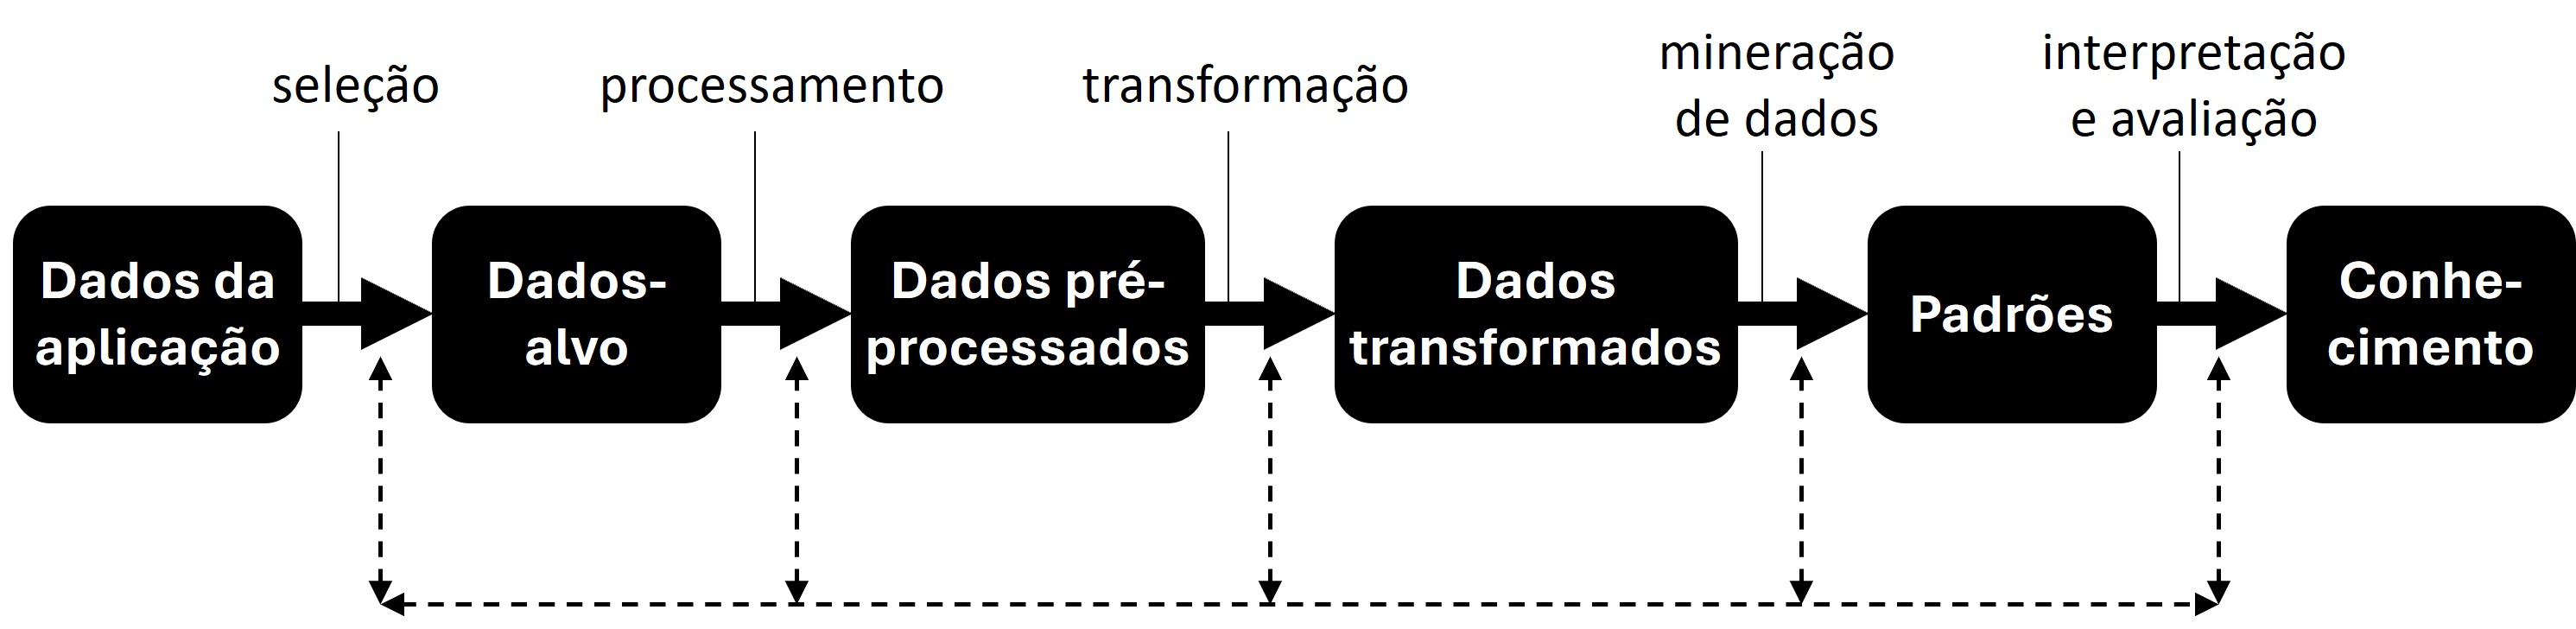
\includegraphics[width=.95\textwidth]{Figures/kdd3.jpg}
    \caption{Diagrama descritivo da metodologia KDD, utilizada neste trabalho}
    \label{fig:kdd}
\end{figure}

% marcos e jackson
\subsection{Base de questões de programação} % pedir revisão para o david

Neste estudo, foi utilizada uma base pública com dados anonimizados de acordo com a Lei Geral de Proteção de Dados (LGPD) do juiz online CodeBench\footnote{\url{https://codebench.icomp.ufam.edu.br/dataset/}}, da UFAM. Ela contém dados de interação de estudantes de 18 cursos de graduação que não pertencem à área de Computação (\textit{non-majors}), matriculados em uma disciplina introdutória de programação. O JO disponibiliza uma IDE para os estudantes elaborarem os códigos de respostas às questões, os quais são avaliados pela ferramenta com respeito aos casos de teste cadastrados pelos instrutores.

As questões foram aplicadas em exames presenciais realizados entre o primeiro semestre letivo de 2016 e o primeiro semestre de 2024, com exclusão dos semestres letivos de 2020, quando outra base de questões foi  aplicada remotamente como avaliação, em função da pandemia de Covid-19. Em seguida, foram excluídas questões que tinham menos de 16 respostas de alunos distintos a fim de reduzir o enviesamento, seguindo a abordagem adotada por \cite{marcos2021}.

Ao final, a amostra deste estudo foi composta por 711 questões resolvidas por 3435 estudantes distintos em laboratório de informática, sob a supervisão de um instrutor e um monitor, de forma a minimizar a troca de códigos entre alunos. Dessa maneira, existe maior probabilidade de cada amostra de código-solução seja única.

%---------------------------------
\subsection{Variáveis independentes e dependentes}

As variáveis independentes usadas como entrada dos modelos de classificação e regressão exprimem a \textbf{complexidade} de uma questão, conforme definida por \cite{pelanek2022complexity}. A complexidade independe da interação do aluno com a questão e consiste em atributos extraídos a partir do código de solução fornecido pelo instrutor no JO, tais como número de operadores e linhas lógicas. Ao todo, foram extraídos 63 atributos de complexidade a partir da base de questões, usando scripts baseados no trabalho de \cite{marcos2021}\footnote{\url{https://anonymous.4open.science/r/questions-irt-calculator-D6DE/README.md}}.

As variáveis dependentes investigadas foram as métricas de \textit{dificuldade} de uma questão, conforme definida por \cite{pelanek2022complexity}. A dificuldade é obtida a partir dos dados de interação dos estudantes com as questões de programação durante a solução delas no IDE fornecido pelo CodeBench. 

Uma vez que não existe um consenso sobre a definição de \say{dificuldade}, foram levantadas 13 métricas que exprimem de alguma forma o esforço médio dos estudantes em resolver cada questão de escrita de código: 12 delas foram tomadas a partir de \cite{jackson2023}, e o presente estudo adicionou o índice de \textit{discriminação}, detalhado na Seção~\ref{sec:calculo_disc}. A Tabela~\ref{tab:metricas_dificuldade} descreve sucintamente cada variável dependente.

\begin{table}[!h]
    \centering
    \scriptsize
    \caption{Variáveis dependentes para expressar a dificuldade de questões}
    \label{tab:metricas_dificuldade}
    \begin{tabular}{lL{.2\textwidth}L{.7\textwidth}}
        \toprule
        \textbf{\#} &
        \textbf{Métrica de dificuldade}             & \textbf{Descrição} \\ \toprule
        M1 & Taxa de acerto               & Razão entre a quantidade de alunos que acertaram a questão e a quantidade de alunos que submeteram a questão pelo menos uma vez \cite{jackson2023}.       \\ \midrule
        M2 & Número de submissões               & Quantidade média de submissões feitas pelos alunos para uma questão. Essa métrica é referida como \say{\textit{attempts}} por \cite{marcos2021}.       \\ \midrule
        M3 & Taxa de aceitação                   & Razão entre o número de submissões corretas e o total de submissões feitas para uma questão \cite{jackson2023}.        \\ \midrule
        M4 & Número de testes                   & Quantidade média de execuções de uma questão usando o ambiente do JO. Adaptação da métrica proposta por \cite{elrik2022}.        \\ \midrule
        M5 & Número de consultas                & Somatório entre o número de submissões e o número de testes da questão. Métrica proposta por \cite{elrik2022}.       \\ \midrule
        M6 & Número de erros de lógica                & Quantidade média de submissões que não passaram em todos os casos de teste, por não terem gerado a saída correta. Métrica proposta por \cite{jackson2023}.       \\ \midrule
        M7 & Número de erros de sintaxe                & Quantidade média de submissões que geraram erro de execução durante os casos de teste. Métrica adaptada por \cite{jackson2023}.     \\ \midrule
        M8 & Número de erros                    & Somatório entre número de erros lógicos e o número de erros de sintaxe.        \\ \midrule
        M9 & Número de eventos                  & Média de linhas do arquivo de log de cada aluno que interagiu com a questão, similar à métrica \say{\textit{events}} de \cite{marcos2021}.       \\ \midrule
        M10 & Número de eventos de deleção       & Média de vezes que as teclas \textit{backspace} e \textit{delete} foram pressionadas durante a resolução da questão. Métrica proposta por \cite{marcos2021}.        \\ \midrule
        M11 & Tempo de implementação             & Tempo médio decorrido entre a primeira interação do aluno com a questão até a primeira submissão correta. Eventos consecutivos com mais de 5 minutos de diferença são descartados e não entram no cálculo desta métrica, por suspeita de inatividade.        \\ \midrule
        M12 & Quantidade de alterações no código & Número de modificações no código entre duas submissões consecutivas, semelhante à métrica \say{\textit{amountOfChange}} usada por \cite{marcos2021}.        \\ \midrule
        M13 & Discriminação                      & Avalia o poder de uma questão em distinguir entre alunos com diferentes níveis de habilidade ou conhecimento.       \\ \bottomrule
    \end{tabular}
\end{table}
    
% jackson 
%---------------------------------
\subsection{Treinamento dos modelos de classificação}

Com base nas escolhas realizadas no trabalho de \cite{jackson2023}, foram utilizados os seguintes modelos de \textbf{classificação}: Support Vector Machine (SVM), Árvores de Decisão (DT), Random Forest (RF), Gradient Boosting (GB) e Extreme Gradient Boosting (XGBoost). Já nos experimentos com \textbf{regressão}, os modelos empregados foram: DecisionTreeRegressor, SVR, NuSVR, RandomForestRegressor e XGBRegressor.

% parágrafo retirado após análise com prof. David
\begin{comment}
Da mesma forma que em \cite{jackson2023}, os modelos baseados em árvores foram escolhidos por apresentarem bom desempenho em bases com estruturas tabulares, com variáveis significativas e sem estruturas temporais ou espaciais multiescalares, enquanto os modelos baseados em vetores de suporte foram escolhidos devido à sua robustez diante de dados de grande dimensão, sobre os quais outras técnicas de aprendizado comumente obtêm classificadores super ou subajustados. Estas serão mostradas na Seção~\ref{sec:metricas_avaliacao}.
\end{comment}

%---------------------------------
\subsection{Cálculo do índice de discriminação} \label{sec:calculo_disc}

A discriminação indica o poder do item em distinguir pessoas com diferentes
níveis de habilidade examinada. Quanto mais próxima for a magnitude de habilidade
que o item puder diferenciar, mais poder o item tem de diferenciar pessoas com habilidades próximas \cite{pasquali2003}. Para calcular a discriminação, adotamos a metodologia utilizada pelo INEP no Exame Nacional de Desempenho de Estudantes (Enade), buscando assim quantificar o poder discriminatório de cada questão. O poder de discriminação de uma questão pode ser medido por meio do coeficiente de correlação ponto-bisserial, que mede a relação entre uma variável dicotômica (acerto/erro da questão) e uma variável numérica (nota final do aluno).

A análise dos resultados obtidos a partir do cálculo da métrica de discriminação evidenciou que grande parte das questões da base apresentava baixo poder discriminatório, revelando um desbalanceamento na base analisada, composta predominantemente por questões de níveis \textit{fácil} e \textit{médio}, com limitada capacidade de diferenciar entre participantes com diferentes níveis de proficiência, conforme ilustrado na Figura~\ref{fig:grafico_freq_discriminacao}.

Com o intuito de adaptar as categorias de discriminação à amostra usadas no presente estudo, foram realizados testes por força bruta, variando-se os limiares de discriminação de forma a obter uma distribuição de frequências mais adequada. O objetivo foi aproximar a classificação das questões a uma divisão em que 70\% das questões pertencem a uma categoria e os 30\% restantes à outra. Tal proporção foi inspirada nos dados apresentados no Relatório da Área de Ciência da Computação do Enade 2021 \cite{enade2021}, que identificou treze objetos com discriminação considerada muito boa e cinco com discriminação boa ou regular, formando dois grupos bem definidos. Como resultado desse processo, foi adotado o limiar de 0{,}09 como ponto de corte, conforme apresentado na Tabela~\ref{tab:discriminacao_prog}.


\begin{table}[!h]
    \centering
    \begin{minipage}[b]{0.52 \textwidth}
        \centering
        \begin{small}
        \caption{Classificação de questões segundo o poder de discriminação. Fonte: \cite{enade2021}}
        \label{tab:discriminacao_inep}
        \begin{tabular}{cc}
            \toprule
            \textbf{Valor de $r_{pb}$} & \textbf{Classificação} \\
            \toprule
            $\ge$ 0{,}40 & Muito bom \\
            0{,}30 a 0{,}39 & Bom \\
            0{,}20 a 0{,}29 & Médio \\
            $\le$ 0{,}19 & Fraco \\
            \bottomrule
        \end{tabular}
        \end{small}
    \end{minipage}
    \hfill
    \begin{minipage}[b]{0.45\textwidth}
        \centering
        \begin{small}
        \caption{Reclassificação de questões segundo o poder de discriminação para a base de questões utilizada.}
        \label{tab:discriminacao_prog}
        \begin{tabular}{cc}
            \toprule
            \textbf{Valor de $r_{pb}$} & \textbf{Classificação} \\
            \toprule
            $>$ 0{,}09 & Fraco \\
            $\le$ 0{,}09 & Muito fraco \\
            \bottomrule
        \end{tabular}
        \end{small}
    \end{minipage}
\end{table}


% explicar como chegamos no número de 0,09

\begin{comment}
\begin{table}[!h]
    \centering
\begin{small}    
    \caption{Classificação de questões segundo o poder de discriminação. Fonte: \cite{enade2021}}
    \label{tab:discriminacao_inep}
    \begin{tabular}{cc}
        \toprule
        \textbf{Valor de $r_{pb}$} & \textbf{Classificação} \\
        \toprule
        $\ge$ 0,40 & Muito bom \\
        0,30 a 0,39 & Bom \\
        0,20 a 0,29 & Médio \\
        $\le$ 0,19 & Fraco \\
        \bottomrule
    \end{tabular}
\end{small}
\end{table}
\end{comment}

\begin{figure}
    \centering
    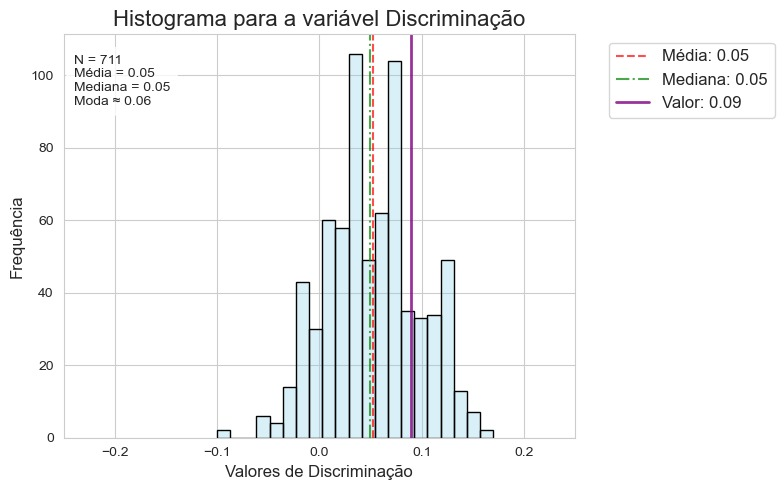
\includegraphics[width=0.90\linewidth]{Figures/discriminacao_freq.jpg}
    \caption{Frequência da discriminação de questões no banco analisado.}
    \label{fig:grafico_freq_discriminacao}
\end{figure}

\begin{comment}
\begin{table}[!h]
    \centering
\begin{small}    
    \caption{Reclassificação de questões segundo o poder de discriminação para a base de questões utilizada}
    \label{tab:discriminacao_prog}
    \begin{tabular}{cc}
        \toprule
        \textbf{Valor de $r_{pb}$} & \textbf{Classificação} \\
        \toprule
        $>$ 0,09 & Fraco \\
        $\le$ 0,09 & Muito fraco \\
        \bottomrule
    \end{tabular}
\end{small}
\end{table}
\end{comment}

% jackson 
\subsection{Métricas de Avaliação}
\label{sec:metricas_avaliacao}

Para avaliarmos a precisão dos modelos com a nova variável --- tanto discriminação quanto taxa de acerto, utilizamos as seguintes métricas: acurácia, precisão, revocação, f1-score (macro) e f1-score (micro). Já na etapa de discriminação, foram utilizadas as seguintes métricas: MAE (\textit{Mean Absolute Error}), RAE (\textit{Relative Absolute Error}), RSE (\textit{Root Squared Error}) e $R^2$ (coeficiente de determinação).

%===========================================================
\section{Resultados e Discussão}
\label{sec:resultados}

A seguir, os resultados obtidos são apresentados e discutidos conforme as questões de pesquisa que nortearam este trabalho.

%-------------------------------------------
\subsection{QP1: É possível prever a discriminação de questões de programação com precisão, a partir de interações prévias dos estudantes?}
\label{sec:resultados_QP1}

Os experimentos detalhados na Seção~\ref{sec:metricas_avaliacao} demonstraram que o modelo Extreme Gradient Boosting obteve o melhor desempenho na predição da discriminação, com um R² ajustado de 0,61. Isso indica que o modelo explica mais da metade da variabilidade dos dados, sugerindo que a discriminação pode ser parcialmente prevista a partir de métricas de interação dos estudantes com o JO durante a resolução das questões.

A Tabela~\ref{tab:tabela_regressao} resume os resultados, destacando que a discriminação superou outras métricas, como taxa de acerto ($R^2$ = 0,48) e tempo de implementação ($R^2$ = 0,52). Além disso, a classificação binária da discriminação alcançou um f1-micro de 0,89 (Tabela~\ref{tab:tabela_class_binaria}), enquanto a classificação ternária apresentou desempenho ainda melhor (f1-micro = 0,90; Tabela~\ref{tab:tabela_class_ternaria}). Esses resultados corroboram a viabilidade da predição, embora com margem para melhorias, conforme discutido na Seção~\ref{sec:limitacoes}.

\begin{table}[h!]
    \centering
    \footnotesize
    \renewcommand{\arraystretch}{1.1}
    \setlength{\tabcolsep}{4pt}
    \caption{Desempenho dos modelos de regressão na predição de métricas de dificuldade, ordenados pelo R² ajustado}
    \label{tab:tabela_regressao}
    \begin{tabular}{@{}llrrrrrl@{}}
        \toprule
        \textbf{\#} & \textbf{Métrica} & \textbf{R²} & \textbf{R² aj.} & \textbf{MAE} & \textbf{RAE} & \textbf{RSE} & \textbf{Modelo} \\
        \midrule
        M12 & Quantidade de alterações no código & 0,70 & 0,69 & 145,55 & 0,56 & 0,30 & Random Forest \\
        M13 & Discriminação & 0,62 & 0,61 & 0,02 & 0,56 & 0,38 & XGBoost \\
        M10 & Número de eventos de deleção & 0,54 & 0,53 & 24,44 & 0,66 & 0,46 & Random Forest \\
        M11 & Tempo de implementação & 0,53 & 0,52 & 133,10 & 0,59 & 0,47 & Random Forest \\
        M4 & Nº de testes & 0,43 & 0,42 & 3,53 & 0,72 & 0,57 & Random Forest \\
        M3 & Taxa de aceitação & 0,43 & 0,42 & 0,09 & 0,75 & 0,57 & XGBoost \\
        M5 & Nº de consultas & 0,42 & 0,41 & 4,50 & 0,73 & 0,58 & Random Forest \\
        M1 & Taxa de acerto & 0,49 & 0,48 & 9,60 & 0,66 & 0,51 & Random Forest \\
        M9 & Nº de eventos & 0,32 & 0,31 & 349,88 & 0,74 & 0,68 & Random Forest \\
        M6 & Nº de erros de lógica & 0,25 & 0,23 & 1,16 & 0,77 & 0,75 & Random Forest \\
        M8 & Nº de erros & 0,21 & 0,20 & 1,49 & 0,78 & 0,79 & Random Forest \\
        M2 & Nº de submissões & 0,19 & 0,18 & 1,47 & 0,80 & 0,81 & Random Forest \\
        M7 & Nº de erros de sintaxe & 0,02 & 0,00 & 0,66 & 0,95 & 0,98 & XGBoost \\
        \bottomrule
    \end{tabular}
\end{table}

\begin{table}[h!]
    \centering
    \footnotesize
    \caption{Resultados da classificação binária (duas classes de dificuldade), ordenados por f1-micro}
    \label{tab:tabela_class_binaria}
    \begin{tabular}{@{}llccl@{}}
        \toprule
        \textbf{\#} & \textbf{Métrica de dificuldade} & \textbf{f1-micro} & \textbf{Acurácia} & \textbf{Classificador} \\
        \midrule
        M13 & Discriminação & 0,89 & 0,83 & Random Forest \\
        M1 & Taxa de acerto & 0,81 & 0,75 & XGBoost \\
        M11 & Tempo de implementação & 0,78 & 0,78 & XGBoost \\
        M12 & Quantidade de alterações no código & 0,77 & 0,77 & Gradient Boosting \\
        M9 & Nº de eventos & 0,73 & 0,73 & Random Forest \\
        M3 & Taxa de aceitação & 0,72 & 0,71 & XGBoost \\
        M5 & Nº de consultas & 0,70 & 0,70 & XGBoost \\
        M8 & Nº de erros & 0,70 & 0,70 & XGBoost \\
        M6 & Nº de erros de lógica & 0,70 & 0,70 & XGBoost \\
        M10 & Nº de eventos de deleção & 0,71 & 0,71 & XGBoost \\
        M2 & Nº de submissões & 0,68 & 0,68 & Gradient Boosting \\
        M4 & Nº de testes & 0,68 & 0,68 & Gradient Boosting \\
        M7 & Nº de erros de sintaxe & 0,65 & 0,65 & XGBoost \\
        \bottomrule
    \end{tabular}
\end{table}

\begin{table}[h!]
    \centering
    \footnotesize
    \caption{Resultados da classificação ternária (três classes de dificuldade) ordenados por f1-micro}
    \label{tab:tabela_class_ternaria}
    \begin{tabular}{@{}llccl@{}}
        \toprule
        \textbf{\#} & \textbf{Métrica de dificuldade} & \textbf{f1-micro} & \textbf{Acurácia} & \textbf{Classificador} \\
        \midrule
        M13 & Discriminação & 0,90 & 0,84 & XGBoost \\
        M11 & Tempo de implementação & 0,67 & 0,67 & Random Forest \\
        M12 & Quantidade de alterações no código & 0,63 & 0,63 & XGBoost \\
        M1 & Taxa de acerto & 0,63 & 0,62 & Gradient Boosting \\
        M9 & Nº de eventos & 0,61 & 0,60 & XGBoost \\
        M3 & Taxa de aceitação & 0,59 & 0,58 & Gradient Boosting \\
        M6 & Nº de erros de lógica & 0,56 & 0,56 & Random Forest \\
        M10 & Nº de eventos de deleção & 0,56 & 0,56 & Gradient Boosting \\
        M4 & Nº de testes & 0,54 & 0,54 & Random Forest \\
        M2 & Nº de submissões & 0,52 & 0,51 & XGBoost \\
        M5 & Nº de consultas & 0,52 & 0,52 & Random Forest \\
        M8 & Nº de erros & 0,50 & 0,50 & XGBoost \\
        M7 & Nº de erros de sintaxe & 0,46 & 0,45 & Gradient Boosting \\
        \bottomrule
    \end{tabular}
\end{table}


%-------------------------------------------
\subsection{QP2: Existe correlação significativa entre discriminação e as demais métricas de dificuldade usadas por \cite{jackson2023}?}
\label{sec:resultados_QP2}

A análise de correlação revelou que a discriminação não apresenta relações fortes com a maioria das métricas de dificuldade\footnote{A matriz de correlação completa pode ser vista em \url{https://anonymous.4open.science/r/questions-irt-calculator-D6DE/README.md.}}. Destacam-se apenas correlações moderadas com:

\begin{itemize}
    \item \textbf{Taxa de acerto} ($-$0,52): Questões mais fáceis tendem a discriminar menos, pois questões muito fáceis (alta taxa de acerto) são acertadas por quase todos os alunos, independentemente de seu nível de habilidade, reduzindo sua capacidade discriminatória \cite{Liz2020}. Isto é corroborado por \cite{pelanek2022complexity}, que destacam que itens muito fáceis ou muito difíceis têm menor poder discriminatório.
    \item \textbf{Taxa de aceitação} ($+$0,44): Maior aceitação está associada a melhor discriminação. Segundo \cite{elrik2022},  questões resolvidas com menos tentativas (alta aceitação) tendem a ser mais claras e objetivas, permitindo que alunos habilidosos se destaquem. Isso está alinhado com a psicometria clássica, que associa itens bem construídos a maior discriminação \cite{Liz2020}.
    \item \textbf{Tempo de implementação} ($-$0,38): Questões mais demoradas discriminam pior.  O tempo de implementação está relacionado à complexidade cognitiva da tarefa \cite{pelanek2022complexity}. Questões que demandam muito tempo podem envolver fatores confundidores (como ambiguidades no enunciado ou complexidade excessiva), que afetam igualmente alunos de diferentes níveis, reduzindo a discriminação. \cite{whalley2014} destacam que tempo elevado nem sempre reflete dificuldade, mas pode indicar problemas de design da questão.
\end{itemize}

Portanto, esses achados sugerem que a dificuldade e a discriminação, embora relacionadas, capturam aspectos distintos da experiência do estudante com a questão.

%-------------------------------------------
\subsection{QP3: O uso de uma base de questões maior melhora os resultados de predição obtidos por \cite{jackson2023}?}
\label{sec:resultados_QP3}
% tempo e david

Este estudo expandiu a base de dados em comparação ao trabalho de \cite{jackson2023}, mas os resultados sugerem que o aumento do volume de questões não eliminou desafios como a baixa discriminação intrínseca das questões (Seção~\ref{sec:calculo_disc}). Apesar disso, o modelo proposto superou benchmarks anteriores em métricas como $R^2$ e f1-micro, indicando que a combinação de técnicas (e.g., Extreme Gradient Boosting) pode compensar limitações amostrais. Contudo, a queda de desempenho na classificação ternária (e.g., taxa de acerto com f1-micro de 0,63 contra 0,81 na binária) reforça a necessidade de otimizações adicionais.

A classificação ternária é mais desejável que a binária para obter maior granularidade das questões, ajudando assim na progressão do aprendizado; atender aos alunos que estão na habilidade média, evitando tédio ou frustração \cite{whalley2014}; ampliar a curva de avaliação e reduzir o seu viés; e ajuda a identificar \textit{gaps} de conhecimento que a classificação binária pode esconder \cite{barbosa2023}.


%-------------------------------------------
\subsection{Limitações} \label{sec:limitacoes}

Como mostrado na Seção~\ref{sec:calculo_disc}, uma limitação enfrentada foi a discriminação baixa na maioria das questões da base usada (Fraco ou Muito Fraco). Tal fato pode ter sido ocasionado pela base de questões conter apenas questões oriundas de disciplinas de programação introdutória, onde o objetivo é familiarizar o discente com as linguagens de programação através de exemplos simples e preceitos básicos, como laços, condicionais e leitura de entradas do usuário. Assim, é plausível assumir a hipótese de que questões introdutórias de programação não são um bom limiar para realizar a classificação de um espaço amostral de alunos, visto que estas não possuem um alto poder discriminatório. %Isto pode implicar que, em uma aplicação real deste sistema, os resultados serem considerados insatisfatórios pelos docentes responsáveis por tais disciplinas.

Outras limitações deste estudo faz jus à ausência de uma análise detalhada de precisão e cobertura por classe, o que poderia ter esclarecido variações de desempenho entre os cenários binário e ternário, especialmente em contextos de desequilíbrio de classes, sendo recomendável que trabalhos futuros considerem métricas específicas, como matriz de confusão e curvas ROC para uma avaliação mais aprofundada. Cabe destacar que tais aprofundamentos foram evitados em razão do limite máximo de páginas imposto para este artigo, o que restringiu a inclusão de análises complementares.

Ademais, outra limitação encontrada foi o número reduzido de questões disponíveis. Como elas são empregadas apenas em atividades avaliativas e são distribuídas aleatoriamente entre os discentes para evitar plágio, algumas são distribuídas com mais frequência do que outras, causando um desequilíbrio na base de dados.

Por fim, outra limitação dos JOs é que eles avaliam apenas se o código gera a saída esperada para os casos de teste. Com isso, soluções estruturalmente muito diferentes podem ser consideradas corretas, desde que produzam a mesma saída, o que obriga o docente a verificar manualmente se o código foi realmente implementado conforme o esperado. %\say{Do ponto de vista pedagógico, códigos poderiam ser avaliados de forma distinta, dependendo do conteúdo trabalhado e dos critérios do avaliador} \cite{barbosa2023}.
Com isso, é possível afirmar que a abordagem utilizada por JOs não avalia critérios pedagógicos de qualidade em um código \cite{francisco-UEFS-2025}.

%===========================================================
\section{Conclusão e Trabalhos Futuros} \label{sec:conclusao}

Este estudo explorou a predição da dificuldade de questões de programação em juízes online, acrescentando a capacidade discriminatória das questões. A pesquisa confirmou que a inclusão dessa métrica melhora a modelagem da dificuldade, destacando-se como um indicador relevante para distinguir alunos com diferentes níveis de habilidade. Os experimentos demonstraram que modelos baseados em aprendizado de máquina, especialmente o Extreme Gradient Boosting, apresentaram os melhores resultados na predição da taxa de acerto e discriminação. No entanto, a precisão dos classificadores variou conforme a granularidade das categorias, sendo mais eficaz na distinção binária (fácil/difícil) do que na classificação ternária.

% parágrafo ocultado por duas razões: lero-lero da seção de limitações e inserção de um novo parágrafo sobre como a discriminação pode construir bancos melhores
\begin{comment}
Entre as principais limitações do estudo, destaca-se o baixo poder discriminatório da maioria das questões analisadas, o que pode estar relacionado à natureza introdutória da disciplina investigada. Além disso, a base de dados utilizada foi restrita a um único juiz online, o que pode limitar a generalização dos resultados.
\end{comment}

No contexto educacional, o cálculo da discriminação pode ser usado para otimizar o banco de questões em três frentes: (i) seleção criteriosa, excluindo ou revisando itens com coeficiente ponto‑bisserial abaixo de um limiar pré-definido; (ii) desenvolvimento de testes adaptativos, onde itens de alta discriminação garantem avaliações mais precisas; e (iii) monitoramento contínuo, permitindo ao professor identificar rapidamente quais questões falham em diferenciar alunos e precisam ser revisadas ou substituídas.

Uma sugestão de trabalho futuro é investigar mais a fundo a queda de desempenho da classificação ternária e buscar alternativas híbridas para tal, visando melhorar a distribuição entre níveis intermediários de dificuldade. Por fim, outro rumo a ser explorado é investigar como o poder de discriminação de uma questão pode variar ao longo do tempo (e.g., devido a mudanças no currículo ou habilidades dos alunos). 
\begin{comment}

Por fim, outro estudo com potencial de ser realizado é investigar como a divulgação prévia do nível de dificuldade para alunos e instrutores influencia o desempenho dos estudantes e a estratégia pedagógica dos discentes.
\end{comment}


%============================================
\section*{Agradecimentos}

Os autores agradecem à Universidade Federal do Amazonas (UFAM) pelo apoio financeiro por meio do Edital 12/2024 -- PROPESP/UFAM, vinculado ao Programa Institucional de Bolsas de Iniciação Científica (PIBIC), que viabilizou a participação de um dos pesquisadores neste estudo.

\bibliographystyle{sbc}
\bibliography{sbc-template}

\end{document}